% 04authored.tex
% 2011/02/28, v3.00 gamma

\chapter{Figures and tables}
\label{figtabchap}

\section{Figures}

The \cambridge\ class will cope with most positioning of your figures.
As captions fall below figures, the figure must be included first,
then the caption, then the label. This is illustrated in Figure~\ref{cantor}.
The \verb"cantor1.eps" file has been called in using \verb"\usepackage{graphicx}"
in the preamble. Note that if you are producing a list of illustrations
(using \verb"\listoffigures"), you need to repeat the caption
(or place a short version) in square braces, but without the full point.
  \begin{figure}
    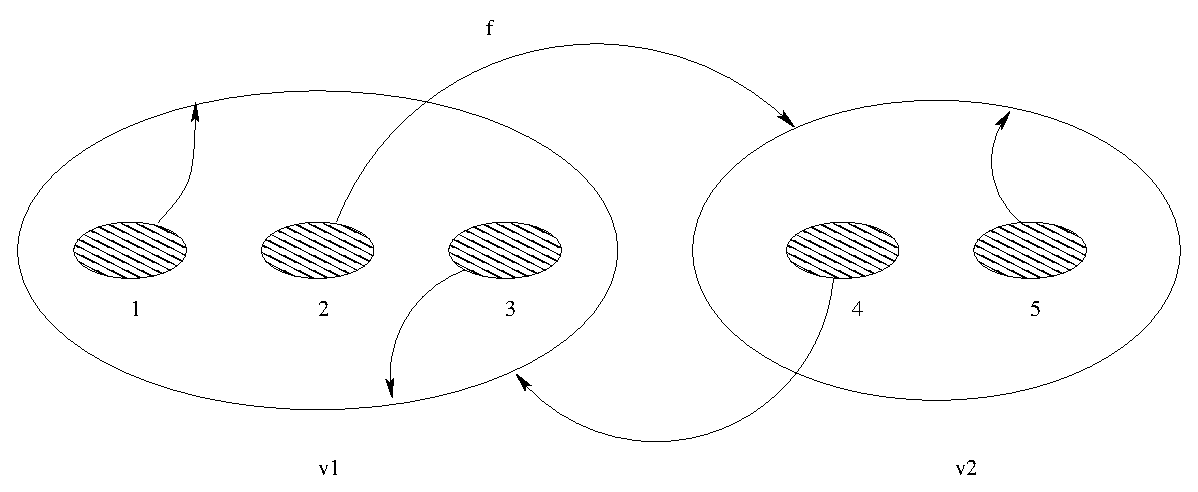
\includegraphics[scale=0.55]{cantor1.eps}
    %  note that the square brace option below is only required
    %  if you intend to produce a list of illustrations
    \caption[Shortened figure caption for the list of illustrations]
      {A Cantor repeller. Long figure captions will be indented left
      and right; short ones will be centred by default.}
    \label{cantor}
\rule[-20pt]{\textwidth}{0.6pt}
\begin{verbatim}
  \begin{figure}
    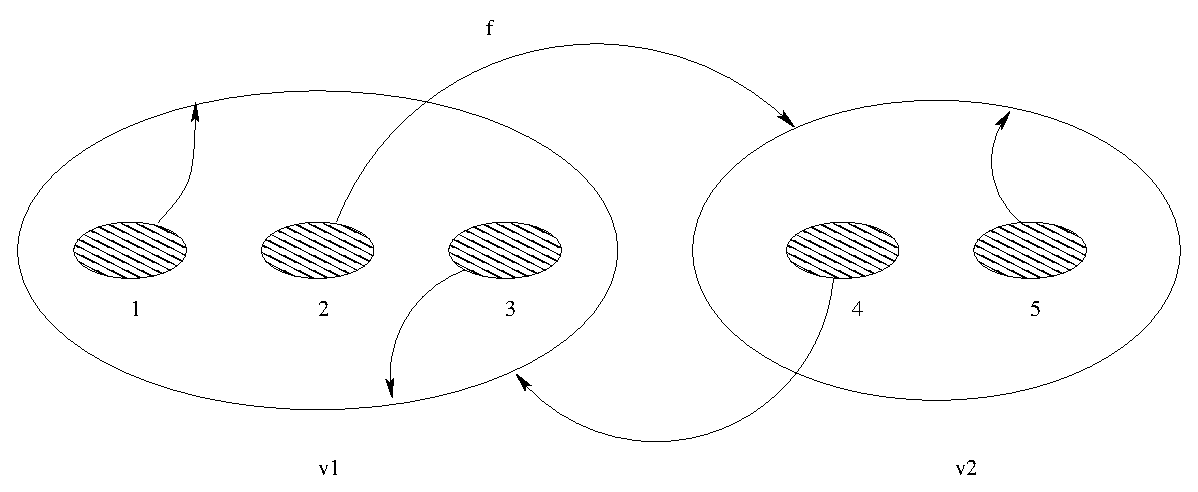
\includegraphics[scale=0.55]{cantor1.eps}
    %  note that the square brace option below is only required
    %  if you intend to produce a list of illustrations
    \caption[Shortened figure caption for the list of illustrations]
      {A Cantor repeller. Long figure captions will be indented left
      and right; short ones will be centred by default.}
    \label{cantor}
  \end{figure}
\end{verbatim}
\rule[20pt]{\textwidth}{0.5pt}
  \end{figure}

\section{Tables}
The \cambridge\ class will cope with most positioning of your tables.
Table captions must be included first, then the label, then the body of the table.
This is illustrated in Table~\ref{sample-table}.
Note that the square brace option below is only required
if you intend to produce a list of tables. You need to use the \verb"minipage"
environment if you have long table captions, or if you have footnotes.

  \begin{table}
    \begin{minipage}{180pt}
    \caption[Shortened table caption for the list of tables]
      {Longer table captions have to be placed inside a minipage,
      otherwise they overhang the table rules.}
    \label{sample-table}
    \addtolength\tabcolsep{2pt}% to stretch columns, if required
      \begin{tabular}{@{}c@{\hspace{25pt}}ccc@{}}
        \hline \hline
        Figure\footnote{\textit{Note:} You must also use a minipage
          environment if you have footnotes.} & $hA$ & $hB$ & $hC$\\
        \hline
        1 & $\exp\left(\pi i\frac58\right)$
          & $\exp\left(\pi i\frac18\right)$ & $0$\\[3pt]
        2 & $-1$    & $\exp\left(\pi i\frac34\right)$ & $1$\\[10pt]
        3 & $-4+3i$ & $-4+3i$ & $\frac74$\\[3pt]
        4 & $-2$    & $-2$    & $\frac54 i$ \\
        \hline \hline
      \end{tabular}
    \end{minipage}
    \rule[-20pt]{\textwidth}{0.5pt}
\begin{verbatim}
  \begin{table}
    \begin{minipage}{180pt}
      %  note that the square brace option below is only required
      %  if you intend to produce a list of tables
    \caption[Shortened table caption for the list of tables]
      {Longer table captions have to be placed inside a minipage,
      otherwise they overhang the table rules.}
    \label{sample-table}
    \addtolength\tabcolsep{2pt}% to stretch columns, if required
      \begin{tabular}{@{}c@{\hspace{25pt}}ccc@{}}
        \hline \hline
        Figure\footnote{\textit{Note:} You must also use a minipage
          environment if you have footnotes.} & $hA$ & $hB$ & $hC$\\
        \hline
        1 & $\exp\left(\pi i\frac58\right)$
          & $\exp\left(\pi i\frac18\right)$ & $0$\\[3pt]
        2 & $-1$    & $\exp\left(\pi i\frac34\right)$ & $1$\\[10pt]
        3 & $-4+3i$ & $-4+3i$ & $\frac74$\\[3pt]
        4 & $-2$    & $-2$    & $\frac54 i$ \\
        \hline \hline
      \end{tabular}
    \end{minipage}
  \end{table}
\end{verbatim}
\rule[20pt]{\textwidth}{0.5pt}
  \end{table}

\subsection{My vertical rules have disappeared}
Vertical rules in tables are not Cambridge house style; {\cambridge}.cls
removes these rules automatically by redefining the \verb"tabular" environment.
Well-organized tables rarely require vertical rules. Where necessary,
grouping can be indicated by the judicious use of extra horizonatal space
(see Section~\ref{addhoriz}). The amended \verb"tabular" also inserts extra
vertical space above and below the horizontal rules produced by \verb"\hline".

Vertical rules can be reinstated, if necessary. Tables will look squashed,
as in the \LaTeX\ book, because the extra vertical space around horizontal
rules will be removed. To reinstate rules globally, add the command
\verb"\reinstaterules" in the preamble; to reinstate rules for an
individual table, place the \verb"\reinstaterules" command
immediately after the relevant \verb"\begin{table}".

The extra space around horizontal rules will also be removed if
you use \verb"array.sty"; you can ignore this effect, because the space
can be reintroduced globally by the typesetters.

\subsection{Adding space between columns}
\label{addhoriz}
You can add space (2pt in this example) between all columns using\linebreak
\verb"\addtolength\tabcolsep{2pt}". If you wanted to expand the space
only between columns~1 and~2, say to~25pt, use
\verb"\begin{tabular}{@{}c@{\hspace{25pt}}ccc@{}}" (see Table~\ref{sample-table}).

\subsection{Adding space between rows}
If you need additional separation between rows (for example,
between rows~2 and~3 in the body of Table~\ref{sample-table}),
adding \verb"[10pt]" immediately after the double backslash at
the end of row~2 will add a 10pt vertical space (the equivalent of
a blank line at this typesize). This method is more controllable
than inserting a horizontal rule.

\section{Landscape figures and tables, using rotating.sty}
Landscape figures and tables are always rotated anticlockwise,
and may be typeset using the \verb"rotating.sty" package with
the \verb"[figuresright]" option. At final make-up stage it is preferable
for landscape pages to fall on verso (left-hand) pages.

In addition to \verb"rotating.sty", include \verb"floatpag.sty" and
the command \verb"\rotfloatpagestyle{empty}". This combination ensures
that headers and footers are removed from the landscape page:
\begin{verbatim}
  \usepackage[figuresright]{rotating}
  \usepackage{floatpag}
  \rotfloatpagestyle{empty}
\end{verbatim}
In some dvi previewers, floats may not appear rotated. If this happens,
you need to convert the dvi file to PostScript or pdf
in order to see the page properly. You can also rotate figures using
the appropriate optional argument in the \verb"\includegraphics" command:
only the illustration is rotated, so running heads are included as usual and captions will
appear at the foot of the figure rather than to the side, both of
which are unsatisfactory in general.

When converting a PostScript file to a pdf file, you may find that
the landscape page comes out upside-down. If this happens, you need
to modify some of the settings in your conversion program.

\subsection{Coding for landscape figures}

Figure~\ref{sidecantor} was produced as follows:
\begin{verbatim}
  \begin{sidewaysfigure}
    \centering
    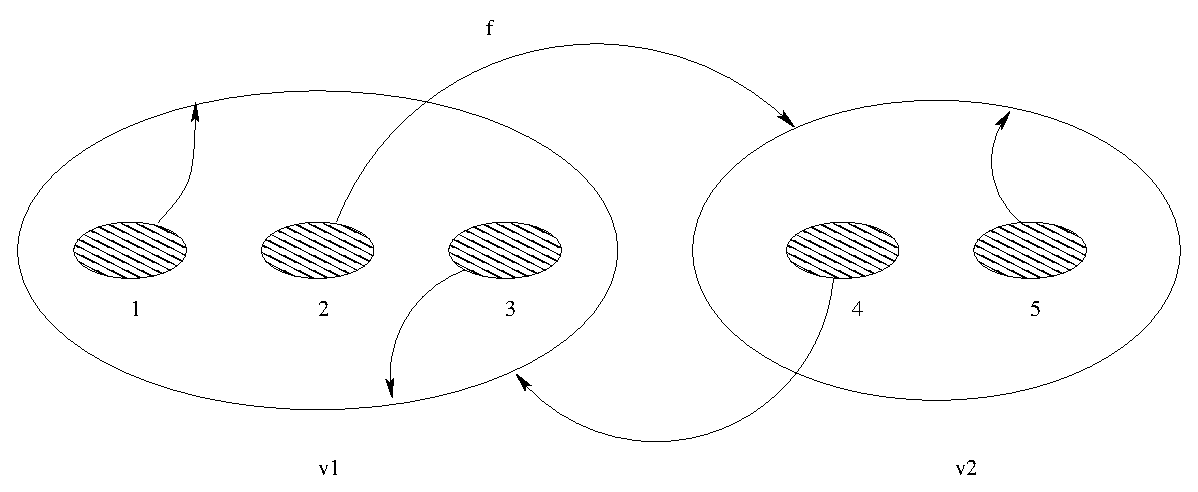
\includegraphics[scale=0.85]{cantor1.eps}
    %  note that the square brace option below is only required
    %  if you intend to produce a list of illustrations
    \caption[Landscape figure]{A Cantor repeller. Figure captions
      will be centred by default.}
    \label{sidecantor}
  \end{sidewaysfigure}
\end{verbatim}
  \begin{sidewaysfigure}
    \centering
    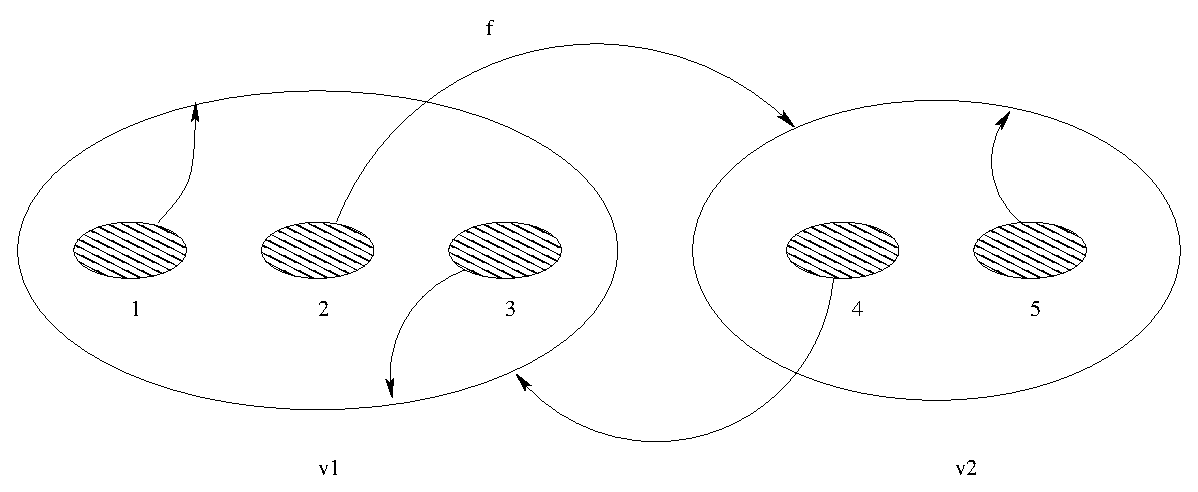
\includegraphics[scale=0.85]{cantor1.eps}
    %  note that the square brace option below is only required
    %  if you intend to produce a list of illustrations
    \caption[Landscape figure]{A Cantor repeller. Figure captions
      will be centred by default.}
    \label{sidecantor}
  \end{sidewaysfigure}


\subsection{Coding for landscape tables}

Table~\ref{sideways} was produced as follows:
%
\begin{smallverbatim}
\begin{sidewaystable}
  \caption[Landscape table]{Grooved ware and beaker features, their finds and
    radiocarbon dates.}
  \label{sideways}
  \addtolength\tabcolsep{-2pt}
  \begin{tabular}{@{}lcccllccccc@{}}
  \hline\hline
  Context & Length & Breadth/  & Depth & Profile & Pottery & Flint & Animal
                                                   & Stone & Other & C14 Dates\\
  && Diameter &&&&& Bones\\[5pt]
  & m & m & m\\
  \hline\\[-5pt]
  \multicolumn{10}{@{}l}{\textbf{Grooved Ware}}\\
  784 & --   & 0.9$\phantom{0}$ &0.18  & Sloping U & P1      & $\times$46
        & $\phantom{0}$$\times$8 && $\times$2 bone & 2150 $\pm$100\,\textsc{bc}\\
  785 & --   & 1.00             &0.12   & Sloping U & P2--4  & $\times$23
                                           & $\times$21 & Hammerstone & -- & --\\
  962 & --   & 1.37             &0.20   & Sloping U & P5--6  & $\times$48
                     & $\times$57 & --& --& 1990 $\pm$80\,\textsc{bc} (Layer 4)\\
  &&&&&&&&&& 1870 $\pm$90\,\textsc{bc} (Layer 1)\\
  983 & 0.83 & 0.73             &0.25   & Stepped U & --     & $\times$18
                                & $\phantom{0}$$\times$8 & -- & Fired clay & --\\
  &&&&&&&&&&\\
  \multicolumn{10}{@{}l}{\textbf{Beaker}}\\
  552 & --   & 0.68             & 0.12  & Saucer    & P7--14 & --           & --
                                                                   & -- &-- &--\\
  790 & --   & 0.60             & 0.25  & U         & P15    & $\times$12   & --
                                                      & Quartzite-lump & -- &--\\
  794 & 2.89 & 0.75             & 0.25  & Irreg.    & P16    & $\phantom{0}$$\times$3
                                                              & -- & -- &-- &--\\
  \hline\hline
  \end{tabular}
\end{sidewaystable}
\end{smallverbatim}
%
\begin{sidewaystable}
  \caption[Landscape table]{Grooved ware and beaker features, their finds and
    radiocarbon dates.}
  \label{sideways}
  \addtolength\tabcolsep{-2pt}
  \begin{tabular}{@{}lcccllccccc@{}}
  \hline\hline
  Context & Length & Breadth/  & Depth & Profile & Pottery & Flint & Animal
                                                   & Stone & Other & C14 Dates\\
  && Diameter &&&&& Bones\\[5pt]
  & m & m & m\\
  \hline\\[-5pt]
  \multicolumn{10}{@{}l}{\textbf{Grooved Ware}}\\
  784 & --   & 0.9$\phantom{0}$ &0.18  & Sloping U & P1      & $\times$46
        & $\phantom{0}$$\times$8 && $\times$2 bone & 2150 $\pm$100\,\textsc{bc}\\
  785 & --   & 1.00             &0.12   & Sloping U & P2--4  & $\times$23
                                           & $\times$21 & Hammerstone & -- & --\\
  962 & --   & 1.37             &0.20   & Sloping U & P5--6  & $\times$48
                     & $\times$57 & --& --& 1990 $\pm$80\,\textsc{bc} (Layer 4)\\
  &&&&&&&&&& 1870 $\pm$90\,\textsc{bc} (Layer 1)\\
  983 & 0.83 & 0.73             &0.25   & Stepped U & --     & $\times$18
                                & $\phantom{0}$$\times$8 & -- & Fired clay & --\\
  &&&&&&&&&&\\
  \multicolumn{10}{@{}l}{\textbf{Beaker}}\\
  552 & --   & 0.68             & 0.12  & Saucer    & P7--14 & --           & --
                                                                   & -- &-- &--\\
  790 & --   & 0.60             & 0.25  & U         & P15    & $\times$12   & --
                                                      & Quartzite-lump & -- &--\\
  794 & 2.89 & 0.75             & 0.25  & Irreg.    & P16    & $\phantom{0}$$\times$3
                                                              & -- & -- &-- &--\\
  \hline\hline
  \end{tabular}%
\end{sidewaystable}

\endinput